\chapter{План Сноевского}

В 1912 году, в «Известиях Отделения русского языка и словесности Императорской Академии наук», томе XVII, книге 3, начиная со страницы 354, ученый-языковед Петр Лазаревич Маштаков опубликовал «План левого берега Днепра от устья реки Десны до устья реки Черторыи» землемера Сноевского, с приложением оного плана вклейкой.

Попади этот план в иную, нуждающуюся в таких знаниях среду, он пророс бы рядом новых исследований, стал одним из краеугольных источников и подспорьем в работе историков, археологов, краеведов. Этого не случилось.  Представляю обиду Маштакова, понимавшего значение предлагаемого им материала.

Публикацию плана Маштаков предварил словами:

\begin{quotation}
«План левого берега Днепра от устья реки Десны до устья реки Черторыи, с показанием селений, островов с озерами и речек луговых», составленный землемером Козелецкого повета Сноевским, хранится в I Отделении библиотеки Академии Наук. По-видимому, он составлен в ответ на запрос о топографии островов, расположенных, против г. Киева. Время его составления, судя по бумаге и почерку, можно отнести к первой половине прошлого столетия. 
\end{quotation}

\newpage

\begin{center}
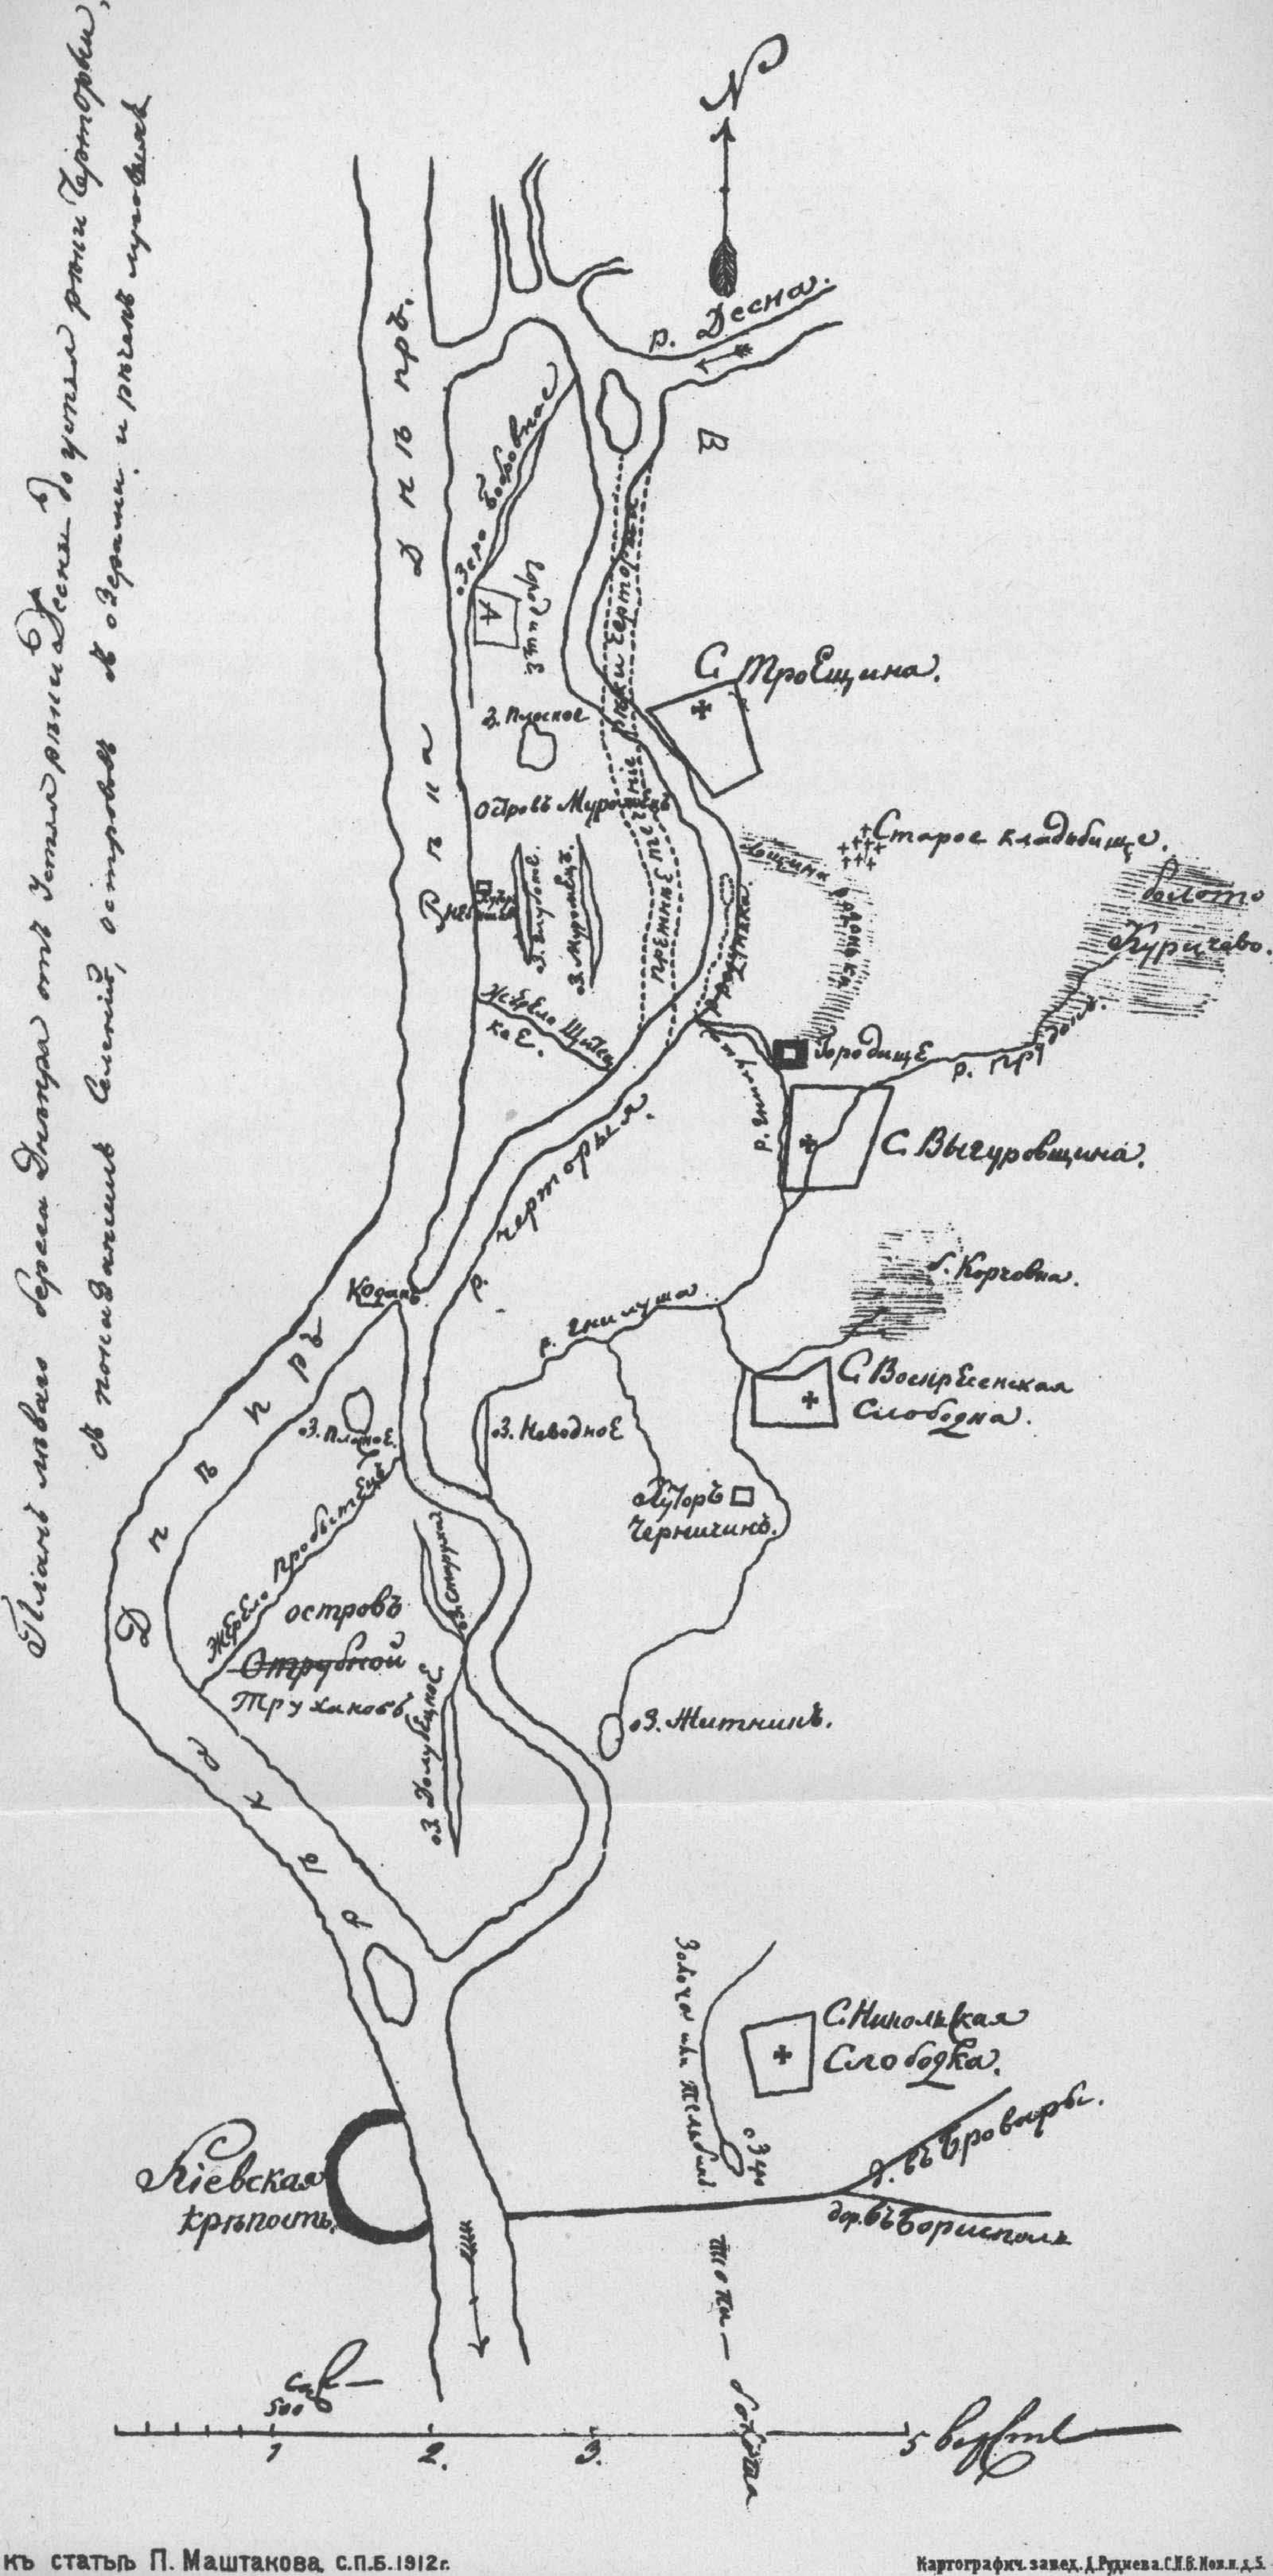
\includegraphics[width=0.82\linewidth]{chast-gorodki/snoev/356a.pdf}
\end{center}

\newpage

К плану прилагалось, от имени Сноевского, пояснение:
 
\begin{quotation}
По показанию старожилых поселян селений: Троещины, Выгуровщины, Воскресенской Слободки, и по распросу некоторых старожилых жителей города Киева, что остров, на котором находится хутор Небышев, название свое имеет по озеру, имеющемуся на нем, – Муромец, равно и тот хутор Небышев ныне называемой имел название по сему острову – Муромец; но когда сим островом владел для сенокосу Киевский комендант Небыш, то и хутор от тех пор таковое название себе получил. Другой же остров, отделяющийся проливом Кодаком, название свое имеет – Отрубной, и сии оба острова, по мнению старожилых людей, составляли в древности один остров Обрубной; ибо когда Черторыя подрезалась близко к Днепру, то бывшею там лощиной Кодаком называемую и прорезалась в Днепр, и старожилыя запомнят, что оной Кодак имел сначала весьма слабое и узкое течение; речька же Черторей в древния времена называлась Восковицей, которая против Троещина\footnote{С падежом всё верно – село тогда называлось Троещино.} имела свое течение, как означено на плане красными чертами\footnote{При публикации стало просто пунктиром.}, и которая быстротой воды, переменяя время от времени свое течение, врезала озерце и речьку Радонку, как на плане значит.

Лугу ж и ручья Ольгова никто из старожилых не знает, а полагают, что сие название лугу и ручья Ольгова от времени забыто, и называется ныне под каким-либо другим именем.

На подлинном подписано:

Повета Козелецкого землемер
Коллежский Ассессор Сноевский.
\end{quotation}

Я хочу обсудить карту и пояснение неотъемлемо с остальным текстом заметки Маштакова из публикации 1912 года.

Маштаков родился в села Кадышевке, Хвалынского уезда Саратовской губернии, в крестьянской семье, в 1872 году. Учил русскому языку в Смольном институте, был преподавателем в гимназии Л. Д.  Леонтьевской в Санкт-Петербурге и на общеобразовательных курсах А. С. Черняева. Получил чин коллежского советника. 

Среди печатных его работ – «Курс русского литературного языка» в трех частях, «К тексту Слова о полку Игореве», другие труды по языкознанию, в особенности по гидротопонимике – названиям рек. Большую часть его наследия уж трудно сыскать: «Список рек Днепровского бассейна» (1913), «Список рек бассейнов Днестра и Буга (Южного)» (1917), «Десна» (1918), «Список рек Донского бассейна» (1934), «Материалы для областного водного словаря» (1931). Умер ученый в феврале 1942 – блокадный Ленинград.

Но мёрзлая зима, когда голод заслонил холод, а дремота переходила в смерть, будет потом, а сейчас 1912 год, Маштаков в расцвете сил, воодушевленно сыплет мыслями о плане Сноевского, дополняя публикацию:

\begin{quotation}
Из «Плана» Сноевского мы можем почерпнуть новые данные для выяснения некоторых темных мест из области исторической географии, и этими данными подтверждаются изыскания П. В. Голубовского о местонахождении летописных оз. Долобского, реки Золотчи, Родуни («Историческая карта Черниговской губернии до 1300 года» в «Трудах XIII Археологического съезда в Екатеринославе 1905 года», т. II), а также и исследование В. Гошкевича о летописном Городце под Киевом («Замок князя Симеона Олельковича и летописный Городец под Киевом». Киев, 1890 г.). Теперь с еще большею уверенностью мы можем утверждать, что 1) село Радунь (Родунь, Радосынь), упоминаемое в Ипатьевской летописи под 1111 и 1151 годами и в Лаврентьевской летописи под 1146 годом, находилось между теперешними селами: Троещиной и Выгуровщиной, на реке Радуньке; 2) там, где на «Плане» находится Городище (рядом с селом Выгуровщиной), находился Городец, упоминаемый в Ипатьевской летописи под 1026, 1135 и 1180 годами, и, вероятно, он же и «Городок Песочный», с которого в 1238 году Менгукан, посланец Батыя, любовался Киевом; 3) Долобьское (Дулебское, Лубейское) оз. Ипатьевской летописи 1111 и 1151 гг. соответствует названному на «Плане» Долубецким; 4) река Золотча (Ипат. летописи под 1151 г.) вытекала из озера Золочи или Тельбень у села Никольской Слободы.

Кроме того на «Плане» Сноевского мы видим Гнилушу, Старое кладбище, озеро Бобровное, р. Прудок (Прудец), бол. Куричево, упоминаемые в актах Киевского Михайловского монастыря (В. Гошкевич, op. cit.); получаем впервые вариант названия для реки Черторыи – Восковица, и, наконец, по этому «Плану» можем восстановить несколько топографических названий, теперь уже утраченных: озеро Неводное, озеро Житник, болото Куричево, проток Кодак, жерело Щитецкое и др.

П. Л. Маштаков
\end{quotation}

Отмечу чрезвычайную осведомленность Маштакова относительно киевских левобережных водоемов и проявленный интерес к Городку.

Но вот Петр Лазаревич говорит про «село Радунь». Однако в летописях нет села Радунь. Есть \textit{название} Родунь. Когда Юрий Долгорукий (Гюрги) в 1151 году на лодьях плывет по Десне из своего Городка Остёрского и потом «сташа в Родуни», то можно заключить, что Родунь – по крайней мере залив Десны, где Гюрги хотел подождать конницу союзников – Половцев. К слову, в распрях 1151 года упомянуты два Городка – один возле Киева, а другой – Остёрский\footnote{В Остре, по улице Сеспеля, поныне есть на холме городище и Юрьева божница – остатки Михайловской церкви, входившей в состав крепости Юрия Долгорукого. Город Остёр же стоит на берегу реки Остёр, это приток Десны.}.

А в 1110 году Владимир Мономах «бяше в Радосыни», и в то же время с этой Радосынью летопись соотносит Городок, то есть Городок находился в Радосыни или около нее.

«Лубейское» вместо «Долобского» я нигде не встречал – неведомый источник Маштакова? 

Маштаков подтверждает планом Сноевского положение, что городище на плане и есть летописный Городец, но ведь на плане обозначено и другое городище – в северной части острова Муромца. Это второе городище (если верно мое сопоставление) в 1980-х заново открыл археолог Сагайдак, уроженец кстати села Троещины.

Датировка плана. Маштаков по бумаге и почерку относит его к первой половине 19 века. Я решил уточнить датировку. Самое простое было установить верхний рубеж, это 1877 год, ибо на плане село Троещина отмечено на Черторые, а не восточнее на материке, где отстроилось после указанного года. Далее, на карте есть Пробитец, а сей проток существовал еще в 1850 году. 

На давность плана указывает и то, что левый берег Киева отнесен к Козелецкому повету – а ведь известно, что позже он долго находился в другой административной единице, Остёрском уезде Черниговской губернии. Слово «повет» использовалось вместо «уезда», когда в 1781 году Малороссийская губерния была упразднена делением на наместничества, и Козелецкий повет вошел в состав Киевского наместничества. В последующих реформах «повет» по привычке был в ходу наряду с «уездом», потихоньку исчезая из обихода к концу 19 века. Сам же Козелецкий повет отошел затем к Черниговской губернии, а левый берег Киева – к ее же Остёрскому уезду, но гораздо проще датировать карту по ее составителю, землемеру Сноевскому!

Я напал на след Сноевского в документе «Ведомость о положении и пространстве города Козельца», опубликованном без даты в сборнике «Чернігівській губернії – 210 років. Збірник документів і матеріалів»\cite{cherndoc01}. В этом небольшом историко-краеведческом очерке есть отсылка ко временному промежутку с 1807 по 1811 год, как к «истекающему» четырехлетию. Следовательно, очерк сочинен между этими годами. Также указано, что городничим при составлении документа был Елинский, а землемером – коллежский асессор Сноевский. Козелецкий городничий Елинский упомянут еще в одном документе, 1810 года. Я не знаю, сколько лет Сноевский занимал должность землемера до и после 1810 года.

План Сноевского казался мне волшебным подарком судьбы, подтвердившим многие мои вычисления и догадки, сделанные на основании изучения имевшихся у меня тогда в малом количестве давних источников и частых вылазок на местность.

Я взял план на вооружение, но задался множеством вопросов.

Сначала на плане было написано «остров Отрубной», затем «Отрубной» похерено и поставлено «Труханов». В описании плана нет «Труханов». Значит, правку внесли в чистовик, той же рукой, но когда уже не было возможности исправить описание. В дошедших до нас документальных источниках «Обрубной» встречается раз, а «Труханов» – многократно. Да и слово «Труханов» сохранилось в живом предании до наших дней. Почему же землемер пишет крайне редкое название острова? И – Труханова ли?

План ориентирован примерно на север – тоже диковинка. Почти все планы Киева времени, приписанного плану Маштаковым, ориентированы на запад. Известное мне исключение – план «Положения местам вокруг Киева» 1753 года полковника де Боскета, тоже тороватый на водоемы, нигде больше не обозначенные.

Далее, почему отражены летописные названия, и они привязаны к более современным? Допустим, по источникам, Радунка встречается в литовско-польских земельных документах, но Золоча? Золоча в документах не упоминается.

Сноевский, чтобы сопоставить Тельбин с Золочей, должен был внимательно изучить по крайней мере Никонов список Повести временных лет, опубликованный в России в 1768 году, который, кроме Ипатьевского и Лаврентьевского (изданных позже), тоже подробно рассказывает о попытках Гюрги (Юрия Долгорукого) форсировать Днепр – по суше перетаскивали лодьи из Долобского озера в Золочу, а из Золочи выплыли в Днепр.

Напрашивалось два варианта. 

Первый – старожилы действительно помнили Тельбин как Золочу. 

Второй – землемер Козелецкого повета Сноевский был на короткой ноге с летописями, изучал их, сопоставлял былое с насущным. И не только с летописями. 

Общее впечатление от плана вообще такое, что над ним работал многознающий энтузиаст-краевед, пользовавшийся полевыми данными и, в гораздо большей степени – широчайшим набором документальных источников. 

Как я узнал позже, документ с упоминанием Восковицы, с показаниями местного рыбака Закгуры, относится к тому же архиву, с которым работал упомянутый Маштаковым Гошкевич. Сия бумага со времен Екатерины II хранилась в недрах Казенной палаты, пока митрополит Болховитинов не отыскал ее там купно с другими документами по землевладениям киевских монастырей 17-18 веков, и не передал оные документы в библиотеку Киевской Духовной Академии – а сделано это было до 1837 года. И в документе Черторыя вовсе не приравнивалась к Восковице. Но мы обсудим это позже.
  
Другие вопросы не давали мне покоя.

Почему Сноевский спрашивал (я тогда еще думал, что Сноевский лично общался с местным населением) у старожилов о луге и ручье Ольгином? Что за луг и ручей, где о нем еще говорится?

Почему на городище острова Муромца (около «озеро Бобровное») написана буква «А», а к северо-востоку от него, справа от начала Черторыи, поставлена буква «В»? Надо думать, существовала расшифровка этих букв, легенда карты. А много ли встречается карт – кроме тех, что помещены в археологические статьи – где отмечены городища?

Вчитаемся в название карты: «План левого берега Днепра от устья реки Десны до устья реки Черторыи». С какой целью Сноевский подробно картографировал именно этот участок? Юг на карте представлен слабо, но нехило – сопоставлением Тельбина с Золочей! Берлинский на такую смелость не пошел, он просто указал на некую левобережную цепь озер примерно напротив Неводницкой переправы. Мол, эти озёра – всё, что осталось от Золочи. А Сноевский указывает речку Тельбин как Золочу, но Тельбин протекает у него сам по себе, в то время как рядом были озера, во всяком случае знаменитое Свят\'ище.

Составителю плана понадобилось – точно как мне в этой книге – сложить картину левобережных рек на определенном отрезке, включая самые скудные притоки, но – в пределах протяженности Черторыи. Остальное составителю не нужно, но всё равно он проявляет глубокие познания, сопоставляя Тельбин с Золочей.

Таким образом план Сноевского, рассуждал я, заключает в себе тайну. Быть может, это часть какого-то исследования, затрагивающего городища, острова Муромец, Труханов, водную систему Черторыи и вероятно летописное село Ольжичи княгини Ольги. 

Причем Сноевский не просто отмечает современное ему положение объектов, но пытается проследить их изменение во времени – хотя казалось бы, зачем это, ежели, как полагал Маштаков, план «составлен в ответ на запрос о топографии островов»? И какое отношение к топографии островов имеют городища, представляющие чисто археологический интерес?

В начальном варианте этой части книги я основательно пользовался «планом Сноевского». Хотя почти сразу заподозрил, что составил его не Сноевский, но этим именем прикрылся некто очень сведущий в вопросе.

План в чем-то верен, в чем-то ошибочен, ибо, как я понимаю теперь, это итог большого, сложного исследования, включающего работу с архивом в том числе и тем, откуда черпал сведения Гошкевич. План отражает не местность в какое-то определенное время, но представление о местности, сложенное на основании документальных источников. 

В графическую основу «плана Сноевского» легла трехверстовка Шуберта середины 19 века, перерисованная лишь в общих чертах и небрежно. Обозначение урочищ на плане выдает знакомство не только с архивом документов 17-18 веков, но кажется принимались во внимание рассуждения из статьи Гошкевича.

Под воздействием размышлений над новыми для меня источниками я постепенно терял доверие к плану как к источнику, и наконец должен был весьма пересмотреть свое историческое видение местности, отринув многие из прежних рассуждений, основанных на плане.

Во время переделки глав я чувствовал обиду, но обида уравновесилась удовлетворением, ведь без пересмотра отношения к плану Сноевского я бы не выверил заново свои рассуждения и не пришел к более верному пониманию сетки левобережных рек, насколько это возможно исходя из наблюдений и документальных источников.

Далее я буду иногда обращаться к плану, однако не в качестве источника, а расценивая его как обобщение некоего исследования. К сожалению, выданного за источник.

Не буду разбирать, что на плане верно, а что ошибочно, оставляю вам сложить мнение самим, но предостерегаю от использования плана как путеводной звезды при толковании источников – звезда может завести не туда.
